\documentclass[11pt]{article}
\usepackage[utf8]{inputenc}
\usepackage{amsmath, amssymb}
\usepackage{graphicx}
\usepackage{hyperref}
\usepackage{geometry}
\usepackage{natbib}
\usepackage{booktabs}
\usepackage{subcaption}
\geometry{margin=1in}
\graphicspath{{figures/}}

\title{Surprisal as the Drive of Subjective Time:\\
A Gauge-Constrained Taxonomy and Its Decisive Test}
\author{Nathan Hangen}
\date{\today}

\begin{document}
\maketitle

\begin{abstract}
A companion formal note shows that any reparameterization-invariant readout of the
proper-time trajectory alone collapses to an endpoint functional, so interior
sensitivity to subjective time requires a path-distinguishing, $\tau$-intrinsic
\emph{drive}; that result is silent on \emph{which} drive. We propose a principled
candidate---the \emph{surprisal} of experience, $s=-\log p$, so that felt duration is
accumulated information, $\Delta P = k\int s\,d\tau$---gauge-invariant by construction.
The paper is built around the single measurement that decides it---a behavioural
contrast that confirms surprisal, selects a rival, or falsifies surprisal outright.
From this single currency we derive a battery of falsifiable predictions: a saturating,
finite-ceiling age curve (with a late-life slowdown variant), an order effect in which
clustered events read longest, a clean separation from contextual-change accounts, and
Weber--Fechner intensity scaling. The evidence that supports it: the age prediction holds
against digitized lifespan data (a plateau to age 94, ruling out proportional and
unbounded laws); in the open Blursday database ($N=2{,}376$) greater \emph{subjective}
confinement predicts a markedly slower momentary passage of time
($p\approx4\times10^{-12}$); and a back-heavy convergence asymmetry emerges in embodied
agents that never read the drive. Where the data already strain it: the
\emph{objective}-mobility version of the locality test is null, and the retrospective arm
is wrong-signed---greater confinement \emph{expands} rather than compresses remembered
duration---so what survives is the narrower claim that felt isolation, not spatial extent,
slows momentary time. Because these consistency checks do not adjudicate surprisal against
its nearest rival, we close with the decisive contrast that does: a single behavioural test
on which surprisal predicts a clustered event-burst reads \emph{longest} while a
contextual-change account predicts \emph{shortest}. A single currency ties subjective time
to its drivers, and we are explicit throughout about where the data strain it.
\end{abstract}

\section{Introduction}
The felt speed of time is not fixed: it stretches under novelty and compresses under
routine, and it changes systematically across the lifespan. A companion formal note
establishes a structural constraint on \emph{any} model of this phenomenon: if the
readout is invariant under reparameterization of physical time and depends on the
proper-time trajectory alone, it is determined by the endpoints of that trajectory
(with or without internal memory). Interior sensitivity---the dependence of felt
duration on \emph{how} an interval was filled---therefore demands a
path-distinguishing, $\tau$-intrinsic input \citep{timeperception2026theorem}.

That theorem is a gate, not a mechanism: it says what a drive must look like, not what
it is. Existing accounts supply drives operationally (a pacemaker rate, an
attentional gate, a count of contextual changes \citep{treisman1963temporal,
zakay1997temporal, block1978remembered}) but leave open \emph{why} those particular
quantities. We propose that the drive is the \emph{surprisal} of experience,
$s=-\log p(\text{event})$ under the observer's predictive model---the information each
moment carries. Surprisal is a single, principled currency; this paper asks what it
predicts and tests one prediction directly. More than a model, it is a model
paired with the single measurement that decides it: \S\ref{sec:decisive} sets out
a behavioural contrast whose outcome confirms surprisal, selects a named rival, or
falsifies surprisal outright---the experiment the paper is built to provoke.

\section{An information-theoretic principle for subjective time}
We state the framework as a principle and develop its consequences; the psychology of
later sections is its instantiation, not its foundation.

\subsection{The principle}
Let a stimulus stream $x(\tau)$ be defined on proper time $\tau$ and let the observer hold
a predictive model $\mathcal{M}_\tau$ whose precision sharpens with experience. With the
surprisal (self-information) $s(\tau)=-\log p\big(x(\tau)\mid\mathcal{M}_\tau\big)$, we
posit that the subjective duration of an interval equals the information registered over it:
\begin{equation}
\Delta P \;=\; k\!\int_{\tau_0}^{\tau_T} s(\tau)\,d\tau \;=\; k\,\mathbb{I}_{[\tau_0,\tau_T]},
\qquad s(\tau) = -\log p\big(x(\tau)\mid \mathcal{M}_\tau\big).
\label{eq:principle}
\end{equation}
Perceived duration is accumulated information; the felt \emph{rate} of time is an
information density. The scale $k$ fixes units (bits to felt time) and is a single
global constant, not a per-prediction knob: every falsifiable consequence below is a
\emph{ratio} (the finite age ceiling, \S\ref{sec:fisher}), an \emph{ordering} (the
reorder effect, \S\ref{sec:predictions}), or a \emph{log-slope} (Weber--Fechner,
\S\ref{sec:predictions}), each invariant under $k\to ck$, so $k$ cannot be tuned to
rescue any one of them. Two facets follow, with opposite sign, and they are the two
empirically established modes of time experience. A \emph{remembered} interval that
registered little information reads as short --- it ``went fast'' (retrospective speed
$\propto 1/\bar s$); a \emph{passing} interval is felt through the rate of information
currently being realized (momentary speed $\propto s$). This is the classical
retrospective/momentary (``holiday paradox'') split, here a single principle viewed two ways.

The principle is not free-standing: surprisal $-\log p$ is the quantity self-organizing
agents are argued to minimize under the free-energy principle \citep{friston2010free}, and
duration models in which perceived time accumulates salient perceptual change or
surprise-gated episodic memories are already established
\citep{roseboom2019activity, fountas2022predictive}---indeed the holiday-paradox reading
above is theirs. We do not claim the accumulation idea as novel. Our contribution is to
(i) place it under the reparameterization-invariance constraint of the companion note, which
selects surprisal (a $\tau$-intrinsic functional) over coordinate-rate drives; (ii) show that
a \emph{single} information currency then also yields the age ceiling (\S\ref{sec:fisher}),
Weber--Fechner scaling (\S\ref{sec:predictions}) and a spatial-locality \emph{prediction}
(\S\ref{sec:capacity})---whose status the data qualify (\S\ref{sec:locality}); and (iii) put
that locality prediction to a direct test. That ``information'' here is a physical, not metaphorical, quantity is
underwritten by the information--thermodynamics correspondence \citep{jaynes1957information,
landauer1961irreversibility}.

\subsection{Gauge invariance (corollary)}
Because $\mathbb{I}$ in \eqref{eq:principle} is a functional of the proper-time data
$(\tau,x(\tau))$ alone, it is invariant under any reparameterization $t\to t'$ of physical
time --- it never reads a coordinate-time quantity. This is exactly the constraint the
companion note proves necessary, and it separates the surprisal drive from
coordinate-surprise foils (which read $d\tau/dt$). Numerically (Fig.~\ref{fig:gauge}) the
drive's response to a battery of time-warps converges to zero under refinement while a
coordinate-dependent observer converges to a nonzero floor.

\paragraph{Which reparameterization (and which it is not).}
The invariance at issue---and the only one the companion note requires---is under
reparameterization of \emph{physical time}, $t\to t'$. It holds for \eqref{eq:principle}
whatever the form of $p$, because $\Delta P$ integrates the scalar density $s(\tau)$
against the invariant measure $d\tau$ along the fixed proper-time trajectory, so a smooth
relabeling of the time coordinate leaves it unchanged; the numerical warp test
(Fig.~\ref{fig:gauge}) certifies exactly this. A \emph{distinct} symmetry---%
reparameterization of the observable itself, $x\mapsto\varphi(x)$---is neither claimed nor
needed, and for a continuous density it does not hold: $-\log p(x)$ then acquires a
Jacobian term $-\log|\varphi'|$. Surprisal is therefore defined relative to a fixed
stimulus encoding (the observable's natural measure). The discrete-token instantiation of
\S\ref{sec:embodied} is automatically invariant on the observable axis (a relabeling only
permutes a probability mass function); in the continuous case, if observable
coordinate-freeness is also wanted, the drive generalizes to a \emph{relative} surprisal---a
Kullback--Leibler divergence against a fixed reference measure---which is coordinate-free by
construction. This is a generalization, not a correction: none of the predictions below
depends on it.

\begin{figure}[t]\centering
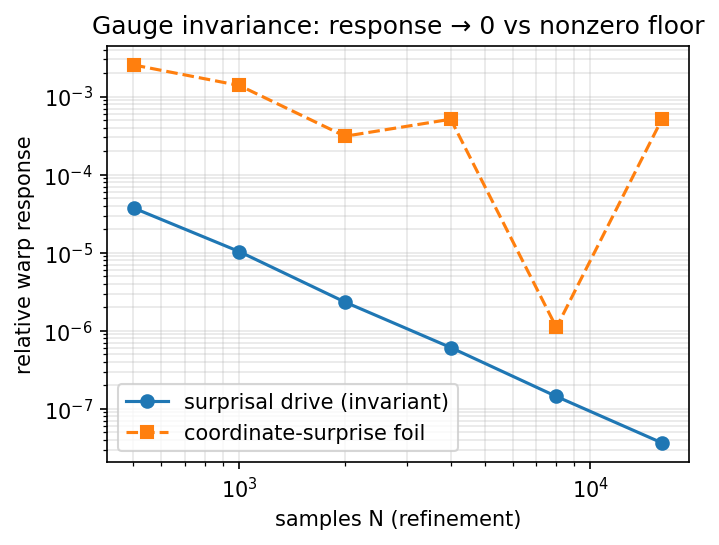
\includegraphics[width=0.6\textwidth]{fig1_gauge_invariance.png}
\caption{Gauge invariance: the surprisal drive's warp response vanishes under refinement
(pure discretization); a coordinate-surprise foil plateaus at a nonzero floor.}\label{fig:gauge}
\end{figure}

\subsection{Missing information, Fisher information, and a finite age ceiling}
\label{sec:fisher}
Let the environment emit $x\sim\mathcal{N}(\mu,\sigma^2)$ with $\mu$ a learnable parameter
and $\sigma^2$ irreducible noise. After experience $a$ (observation count) the observer's
posterior over $\mu$ has variance $v(a)=(\lambda_0+a\,\mathcal{I}_F)^{-1}$, where
$\mathcal{I}_F=\sigma^{-2}$ is the per-observation Fisher information: \emph{Fisher
information accumulates linearly with experience, and missing information about the
learnable structure falls as $\tfrac12\log v(a)\sim-\tfrac12\log a$}. The one-step
predictive variance is $\sigma^2+v(a)$, so the expected surprisal rate is the predictive
entropy
\begin{equation}
r(a)=\tfrac12\log\!\big(2\pi e\,[\sigma^2+v(a)]\big)
\;\xrightarrow[a\to\infty]{}\;\tfrac12\log\!\big(2\pi e\,\sigma^2\big)\equiv r_\infty .
\end{equation}
The rate does not vanish: the learnable missing information disappears ($v\to0$) but the
\emph{irreducible} missing information set by $\sigma^2$ remains. Hence the retrospective
felt speed $s(a)\propto r(\text{ref})/r(a)$ rises and \textbf{saturates at a finite ceiling}
$r(\text{ref})/r_\infty$. The saturating age curve is therefore not assumed: it is the
signature of Fisher-information accumulation against a noise floor. Strict proportionality
has no floor, predicts unbounded speed-up, and is the law the lifespan data reject
(\S\ref{sec:predictions}).

\subsection{Entropy capacity and locality}
\label{sec:capacity}
A locality affording $W(\ell)$ distinguishable states bounds the entropy of the observation
distribution by $\log W(\ell)$ (maximum entropy at fixed support \citep{jaynes1957information}), and hence bounds the
achievable information rate, $r \le \log W(\ell)$ per unit time. The realized momentary rate
is $\rho\,\log W(\ell)$ with an engagement fraction $\rho\in[0,1]$: \emph{locality sets the
ceiling on information rate; attention/boredom sets the fraction realized}. Shrinking the
locality (confinement, $W\!\downarrow$) lowers the ceiling, and monotony lowers $\rho$; both
reduce accrued information and---by \eqref{eq:principle}---slow the felt passage of time.
This is a state-counting (Boltzmann) bound: ``the size of a region bounds the information
experienced in it'' already at the level of accessible microstates, with no appeal to
anything exotic. We flag in advance that the test in \S\ref{sec:locality} supports the
\emph{momentary slowing} but \emph{not} the capacity ($W$) reading: an objective-mobility
proxy for $W$ is null, implicating the engagement term $\rho$ rather than spatial capacity.

\subsection{Outlook: information and area (conjecture, not load-bearing)}
The strongest ``information $\le$ area'' statement in physics is the Bekenstein/holographic
bound, $S\le A/4\ell_P^2$ \citep{bekenstein1981}. It is tempting to read perceived time ---
accumulated information along a worldline --- as ultimately area-bounded. We record this only
as a conjecture: the bound is not operative here (information registered by an observer sits
dozens of orders of magnitude below it), so it constrains nothing measurable. It would
graduate from analogy to physics only given a \emph{derived} relation between
worldline-accumulated surprisal and a geometric/area quantity of the relevant region, which
we do not have. Nothing in \S\S\ref{sec:fisher}--\ref{sec:capacity} or below depends on it.

\section{Predictions}\label{sec:predictions}
The surprisal drive is not free of structure; it makes specific, falsifiable
predictions, each implemented as an additive simulation.

\paragraph{Age: a finite ceiling, and a late-life slowdown.}
As the predictive model absorbs the learnable structure of the world, surprisal per
unit time declines toward an irreducible floor (the world is never fully predictable),
so a fixed interval carries less surprisal with age and feels faster---and the speed-up
\emph{saturates} at a finite ceiling rather than growing without bound
(Fig.~\ref{fig:age}). Digitized lifespan data \citep{wittmann2005age} show exactly this:
the felt speed of the ``last ten years'' rises steeply to age $\sim$50 and then
plateaus to age 94. Fit against the candidate family, the saturating law wins
decisively while strict proportionality ($s\propto\mathrm{age}$) over-predicts
threefold and is rejected; a logarithmic law is admissible in range but, lacking a
ceiling, diverges from the saturating law only in the oldest tail
(Fig.~\ref{fig:laws}). A variant in which surprisal \emph{rises again} in very old age
(disrupted routine, lost mastery) yields a peak-then-slowdown curve, reproducing
reports that momentary time slows after $\sim$75 \citep{droitvolet2019slows}.

\begin{figure}[t]\centering
\begin{subfigure}{0.49\textwidth}\centering
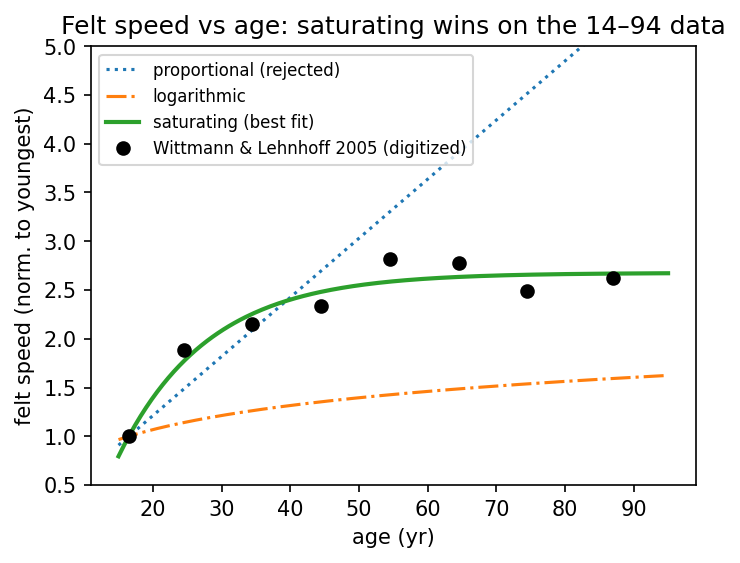
\includegraphics[width=\textwidth]{fig2_age_laws_data.png}\caption{}\label{fig:laws}
\end{subfigure}\hfill
\begin{subfigure}{0.49\textwidth}\centering
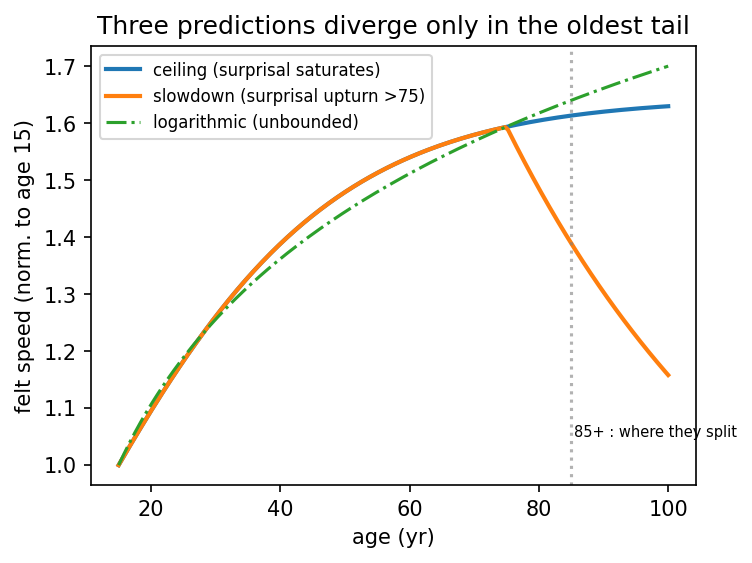
\includegraphics[width=\textwidth]{fig3_ceiling_vs_slowdown.png}\caption{}\label{fig:age}
\end{subfigure}
\caption{(a) Candidate felt-speed laws against digitized lifespan data
\citep{wittmann2005age}: saturating wins; proportional and logarithmic miss.
(b) Ceiling, slowdown, and logarithmic laws diverge only in the oldest tail.}
\end{figure}

\paragraph{Temporal reorder: clustered events read longest.}
For a fixed set of events, only their arrangement is varied. The surprisal drive
predicts that a dense mid-interval burst---maximally surprising against a settled
baseline---reads as the longest, robustly across encoding (Fig.~\ref{fig:reorder}).
The front-versus-back contrast is encoding-dependent and does not cleanly adjudicate
the model; clustered-versus-dispersed is its signature.

\paragraph{Separation from contextual-change.}
A dense burst is maximally \emph{surprising} (surprisal $\to$ long) yet occupies
\emph{few distinct contexts} (contextual-change $\to$ short): the two accounts are
anti-correlated on clustering and thus cleanly distinguishable by a single question
---does a dense burst after calm feel long or short? (Fig.~\ref{fig:reorder}).

\begin{figure}[t]\centering
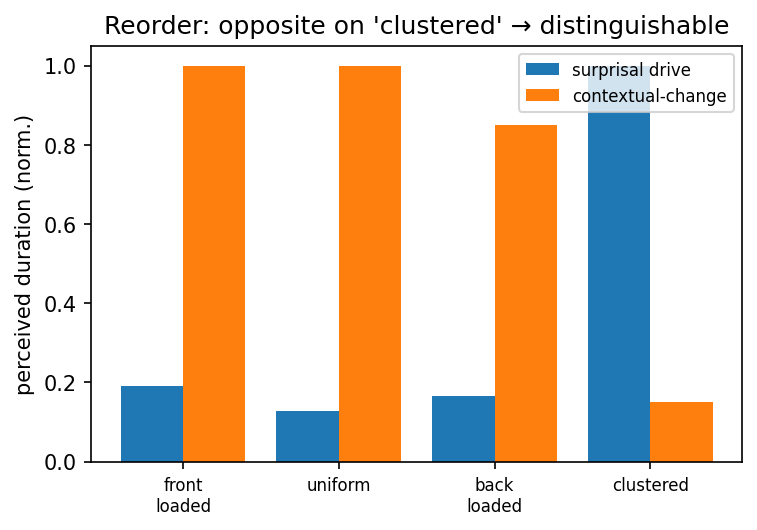
\includegraphics[width=0.6\textwidth]{fig4_reorder.png}
\caption{Reorder: the surprisal drive and a contextual-change account predict opposite
signs on clustered arrangements, so the contrast both defines surprisal's fingerprint
and separates it from its nearest rival.}\label{fig:reorder}
\end{figure}

\paragraph{Weber--Fechner from the same currency.}
If stimulus intensity carries a scale-free prior $p(I)\propto 1/I$ (the
maximum-entropy prior for a positive scale variable), then surprisal
$-\log p(I)=\log I + \mathrm{const}$ is exactly Fechner's logarithmic magnitude, and
its differential gives Weber's constant $\Delta I/I$ (Fig.~\ref{fig:wf}). This is the
efficient-coding account of Weber--Fechner \citep{laughlin1981simple}, recovered here from
the same surprisal currency: the currency that drives subjective time also predicts the
classic intensity law, with no extra assumption beyond the prior.

\begin{figure}[t]\centering
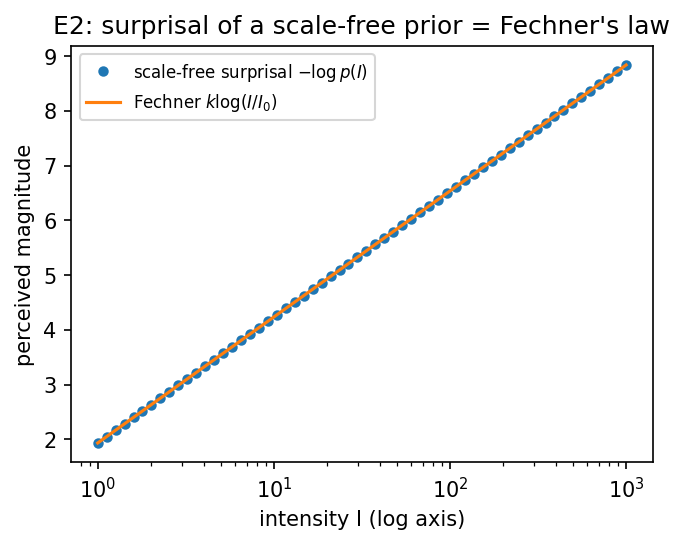
\includegraphics[width=0.55\textwidth]{fig5_weber_fechner.png}
\caption{Scale-free surprisal equals Fechner's log-magnitude; Weber's law is its
differential.}\label{fig:wf}
\end{figure}

\paragraph{Clinical signatures: a passage/estimation dissociation.}
Conditions that alter the predictive machinery should distort subjective time in
specific, falsifiable directions. Driving the same online learner with three altered
parameters---engagement $\rho$ (the fraction of events registered), arousal (pacemaker
rate), and precision---and reading out both the momentary passage (the surprisal rate)
and an explicit attentional clock reproduces the directional signs reported across three
clinical literatures (Fig.~\ref{fig:clinical}). Depression, modeled as reduced
engagement, slows the felt \emph{passage} of time while leaving explicit duration
\emph{estimation} intact---the dissociation found meta-analytically
\citep{thones2015} ($g=0.66$ slower passage; estimation tasks null). A single
accumulated-surprisal clock cannot produce this dissociation, but the two readouts can:
$\rho$ gates the passage accumulator, not the explicit clock. Heightened arousal (mania)
speeds the internal clock, predicting the shorter interval reproductions of manic
relative to depressed patients \citep{mahlberg2008}. Aberrant, unstable precision
(aberrant salience) degrades timing \emph{precision} far more than accuracy, matching the
schizophrenia meta-analysis \citep{thones2017} (variability $g>1$; accuracy effects small)
under the aberrant-salience account of psychosis \citep{kapur2003}. These are consistency
results rather than new data, and the separate attentional clock is the standard
scalar-timing account; the contribution is that one currency plus an attentional clock
predicts the \emph{pattern} of distortions---and, in depression, the dissociation---across
conditions, falsifiable per condition by its sign.

\begin{figure}[t]\centering
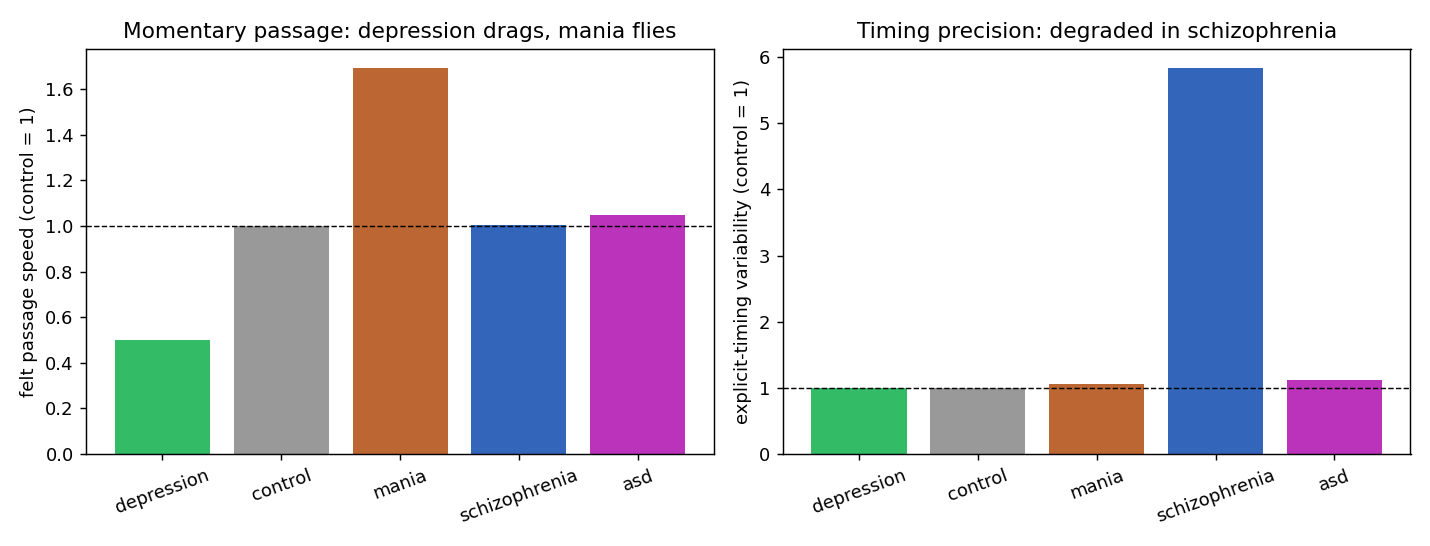
\includegraphics[width=\textwidth]{fig8_clinical.png}
\caption{Predictive-processing clinical signatures (control $=1$). Left: felt passage
speed---reduced engagement (depression) drags, heightened arousal (mania) flies. Right:
explicit-timing variability---degraded under aberrant precision (schizophrenia) while
depression's explicit timing is intact (the passage/estimation dissociation).}\label{fig:clinical}
\end{figure}

\section{Embodied agents: an emergent convergence asymmetry}\label{sec:embodied}
This section is a method as much as a result: \emph{computational psychophysics of
time}---synthetic subjects whose time-perception signatures emerge as byproducts of
prediction, with no human-data bottleneck. The method has two design rules, both
enforced here. The observer is \emph{passive}: the agents optimize their own
objective and never read the surprisal, so any time signature is a byproduct, not a
built-in. And non-circularity is \emph{enforced}: a probed and an unprobed agent
sharing a seed follow identical trajectories, so attaching the readout cannot
perturb what it measures. Within those rules the drive is fixed in advance and the
subject is run, not fit.

The predictions above treat surprisal as a closed-form functional we write down.
A stronger test is whether the same signatures \emph{emerge} when the surprisal
readout merely observes an agent built for a different purpose. We attach the
identical online learner as a \emph{passive} observer to autonomous programs in a
deterministic 3D survival simulation: the agents optimize energy and survival via
their own policies and never read the surprisal, so any time-perception signature
is a byproduct, not a built-in. (A probed agent and an unprobed agent with the same
seed follow identical trajectories, enforcing non-circularity.)

\paragraph{An identical event is more surprising later (back-heaviness).}
The central emergent result is one the closed-form reorder model of
\S\ref{sec:predictions} cannot produce, because that model assigns each event a
\emph{fixed} surprisal independent of when it occurs. In a genuine learner the
predictive variance shrinks as structure is absorbed---$pv_t=\sigma^2+1/\tau_t$
with $\tau_t=\tau_0+t/\sigma^2$---so the surprisal of a fixed deviation $\delta$,
$\tfrac12\log(2\pi\,pv_t)+\tfrac12\,\delta^2/pv_t$, \emph{increases} with experience
for any salient event ($\delta^2>pv_t$) and saturates at
$\tfrac12\log(2\pi\sigma^2)+\tfrac12\,\delta^2/\sigma^2$. The same identical event
thus lands harder the later it occurs, against a more confident model
(Fig.~\ref{fig:backheavy}): the embodied agent reproduces this closed-form
expectation, and the effect holds in $100\%$ of conditions across seeds and a wide
range of predictor priors. This refines the reorder prediction: the front-versus-back
axis is not merely encoding-dependent noise but carries a systematic back-heavy
component in any predictive learner, and the saturation is the same mechanism that
produces the age ceiling (\S\ref{sec:predictions}).

\begin{figure}[t]\centering
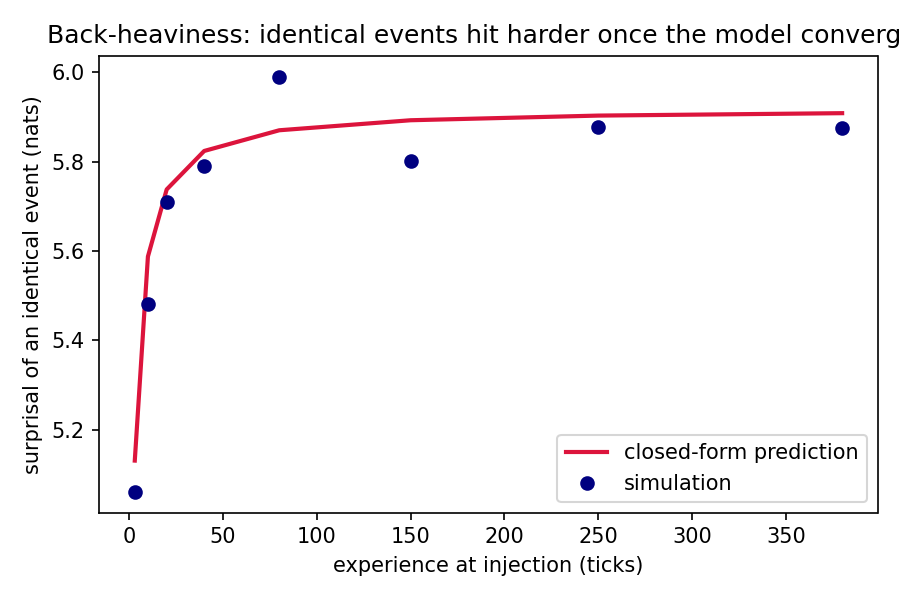
\includegraphics[width=0.6\textwidth]{fig9_back_heaviness.png}
\caption{An identical event injected at increasing experience becomes more
surprising and then plateaus; the embodied simulation (points) tracks the
closed-form expectation (line). This convergence asymmetry is derivable in closed
form and absent from a fixed-per-event accumulator.}\label{fig:backheavy}
\end{figure}

\paragraph{What survives embodiment, and what does not.}
Aggregating the same per-tick surprisal streams under the candidate readouts
(Fig.~\ref{fig:readout}), the clustered burst still reads long under the surprisal
drive---consistent with the fingerprint of \S\ref{sec:predictions}---and a leaky
(recency-weighted) readout makes back-loaded arrangements longest. But the
convergence asymmetry dominates all of them: back-loaded exceeds front-loaded
across pure, leaky, and pacemaker readouts, so the abstract front/back
\emph{opposition} between recency and arousal accounts does not survive embodiment.
We report two honest negatives rather than tuning them away. First, a forward
(pacemaker) kernel does not flip the ordering to front-longest, because the
surprisal substrate is itself back-heavy. Second, a crude embodied
contextual-change readout did not reproduce clustered-\emph{shortest} at any
temporal resolution---the convergence asymmetry again dominated---so the clean
clustered anti-correlation that motivates the decisive test (\S\ref{sec:decisive})
remains an abstract-model prediction to be settled by the human experiment, not an
embodied result. Relatedly, an environmental-volatility$\to$felt-time dose-response
is positive but \emph{weak} on volatility measures computed independently of the
surprisal stream (Spearman $\rho\approx0.4$, seed-dependent; a naive axis derived
from the surprisal stream itself inflates this to $\approx0.8$ and should not be
trusted)---consistent with the engagement-not-capacity reading of the locality
result below.

\begin{figure}[t]\centering
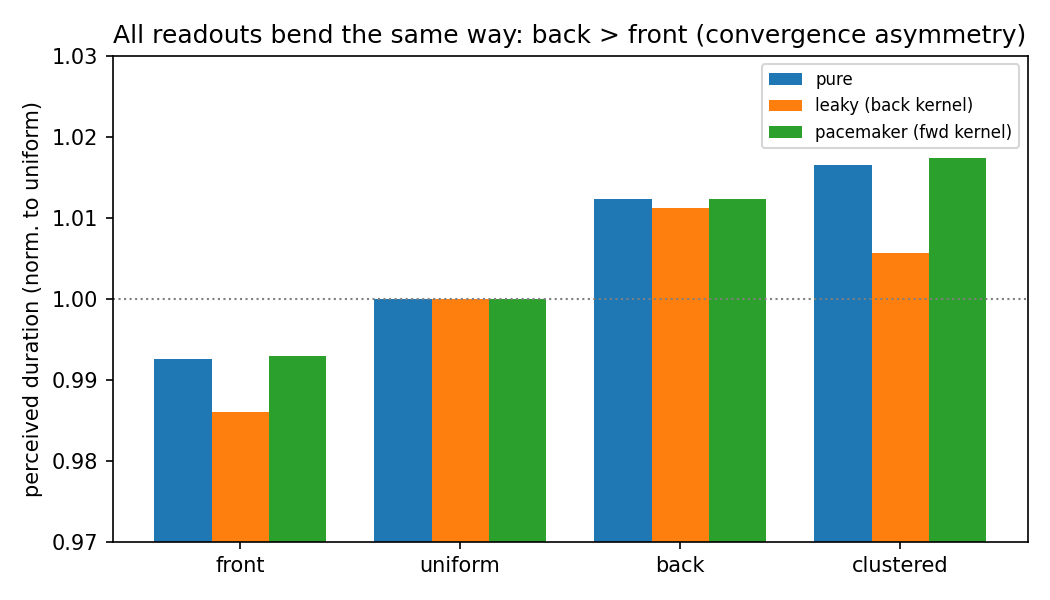
\includegraphics[width=0.6\textwidth]{fig10_readout_contrast.png}
\caption{Perceived duration (normalized to uniform) under pure, leaky, and
pacemaker readouts of the same embodied event streams. All show back $>$ front---the
convergence asymmetry---so the abstract front/back opposition does not survive
embodiment; the clustered burst still reads long.}\label{fig:readout}
\end{figure}

\paragraph{A content footprint in human data.}
Independently of the simulation, the surprisal account predicts that perceived
duration is driven by stimulus \emph{content}, not elapsed time alone. In the
public prospective dataset of \citet{fountas2022predictive} (the model of
\citet{roseboom2019activity}; $6{,}023$ trials, $33$ natural-scene videos), after
regressing each estimate on the true duration, the \emph{identity} of the video
still explains residual variance: per-video bias spans $-2.1$ to $+1.8$\,s
(permutation $p=0.001$), alongside the expected central-tendency bias (slope $0.74$)
and a counting-reduces-overestimation effect. Content biases felt duration beyond
clock time, in humans. This is necessary but not sufficient---it is consistent with
any content-driven account and re-confirms an established finding; the decisive,
uniquely-surprisal test (whether our per-video surprisal predicts \emph{which}
videos are over-estimated) is blocked because the stimulus videos were never
released.

These are synthetic subjects: the readout is the theory, so the contribution is a
mechanistic existence proof and a sharp prediction---the closed-form,
embodiment-robust back-heaviness---rather than human validation of the drive.

\section{A first empirical test: locality slows felt time}\label{sec:locality}
The drive's hard-to-observe quantity is the surprisal/novelty \emph{rate}. We propose
that the spatial extent a person inhabits---their \emph{locality}---is an observable
proxy: a smaller locality (confinement, routine) delivers less novelty per unit time.
The momentary prediction is then that smaller locality \emph{slows} felt time
(monotony drags), the retrospective prediction that it \emph{compresses} remembered
duration (few memorable events).

We test the momentary arm in the open Blursday database \citep{chaumon2022blursday},
in which COVID-19 lockdowns acted as a natural manipulation of locality. Regressing the
felt passage of time (a $0$--$100$ visual-analog scale, $0=$ very slow) on a
self-reported subjective-confinement index, with age, session, and country covariates
and country-clustered errors (Fig.~\ref{fig:loc}), we find that greater confinement
predicts a slower passage of time: $\beta = -1.11$ scale points per confinement-index
unit ($p\approx4\times10^{-12}$; $N=2{,}376$ observations, $1{,}899$ participants, $9$
countries), about $-17$ points across the observed confinement range. The direction and
magnitude match the prediction and the broader lockdown literature, in which boredom and
inactivity---the locality$\to$novelty pathway---mediate the effect.

\begin{figure}[t]\centering
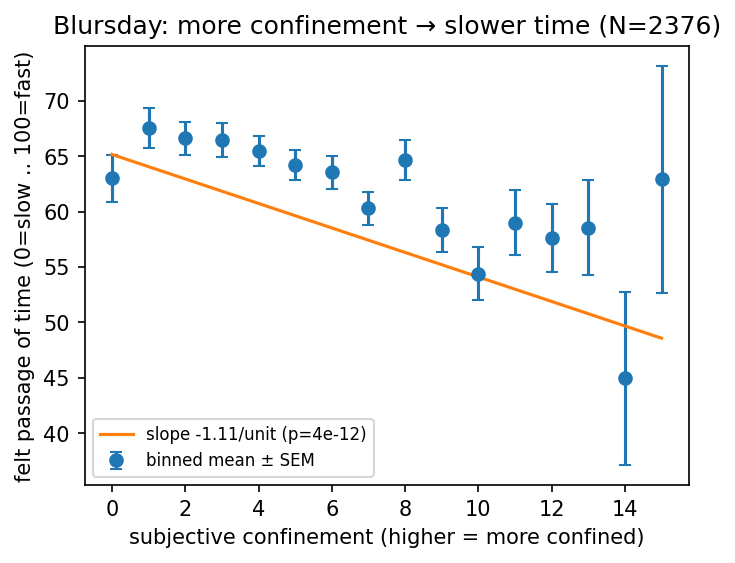
\includegraphics[width=0.6\textwidth]{fig6_blursday_locality.png}
\caption{Blursday ($N=2{,}376$): greater subjective confinement predicts a slower felt
passage of time (binned means $\pm$ SEM; cluster-robust slope).}\label{fig:loc}
\end{figure}

Two sharper follow-ups, however, qualify this and partly contradict the
\emph{spatial} reading. (i) Replacing the subjective index with an \emph{objective}
transit-mobility index (Google) yields a null effect ($\beta=+0.016$, $p=0.80$; null
with or without session controls, and mobility is $\sim\!0.8$ collinear with lockdown
phase): the strong effect rides on \emph{felt isolation}, not measured movement.
(ii) The retrospective arm runs the wrong way: greater confinement \emph{expands}
remembered duration (log estimate/actual, $\beta=+0.004$, $p=0.002$, $\sim\!+6\%$ across
the range), the opposite of the predicted compression---though consistent with reports
of time ``stretching'' during lockdown. So what survives is narrower than the spatial
hypothesis: subjective confinement slows \emph{momentary} felt time, robustly, but the
objective-locality (state-counting) prediction of \S\ref{sec:capacity} is not supported
and the retrospective prediction fails. In the $r=\rho\log W$ decomposition this points
to the \emph{engagement} term $\rho$ (boredom/inactivity), not the capacity $W$, as the
operative variable---a framework-consistent reading, but one the spatial framing did not
anticipate.

\paragraph{A regime the readout cannot reach.} A companion simulation asks whether the
model's retrospective readout could even produce a confinement-driven distortion in this
regime. It cannot: the confinement--distortion slope collapses from $-0.73$ under varied
surprise to $\approx 0$ once surprise is floored, and the interior distortion vanishes for
a single undifferentiated interval, growing only once the interval carries several
distinguishable segments. Lockdown confinement is plausibly both floored and
undifferentiated, so the observed retrospective \emph{expansion} is most consistent with an
exogenous (emotional/anchoring) effect on which the surprisal readout is silent in that
regime, rather than a refutation of the account. This does not settle the arm; it delimits,
computationally, the conditions under which the account makes a retrospective prediction at
all.

\section{The decisive test (preregisterable)}\label{sec:decisive}
The consistency checks above do not \emph{adjudicate} surprisal against its nearest rival,
because most accounts predict the same sign on most manipulations. One contrast does
separate them. Under surprisal, a dense burst of events after a calm baseline is maximally
informative and reads as the \emph{longest} interval; under a contextual-change account,
the same burst occupies the \emph{fewest} distinct contexts and reads as the
\emph{shortest}. In simulation the two are essentially anti-correlated on this clustered
contrast (normalized clustered-vs-dispersed score $+0.96$ surprisal vs $-0.94$
contextual-change; \S\ref{sec:predictions}). The experiment is therefore a single,
high-powered question.

\paragraph{Design.} Within-subject; matched event sets ($n$ events, fixed total, fixed
interval endpoints) presented in four arrangements---front-loaded, uniform, back-loaded,
and clustered (a dense mid-interval burst). DV: perceived interval duration (reproduction
and a 2AFC replication). Stimulus information/change content is logged per trial (a
model-based surprisal stream) as a covariate.

\paragraph{Preregistered predictions.} (a) \emph{Surprisal:} clustered $>$ dispersed
arrangements (clustered longest). (b) \emph{Contextual-change:} clustered $<$ dispersed
(clustered shortest). (c) \emph{Leaky-accumulator / pacemaker:} ordered front/back effects
with clustered intermediate. The clustered-vs-dispersed \emph{sign} is the decisive
quantity; the front/back axis is not (it is encoding-dependent for surprisal,
\S\ref{sec:predictions}).

\paragraph{Decision rule \& falsifier.}
\begin{center}
\fbox{\parbox{0.92\linewidth}{\centering
Clustered rated \emph{longest}, effect scaling with the burst's logged surprisal $\Rightarrow$ \textbf{surprisal}.\\[2pt]
Clustered rated \emph{shortest} $\Rightarrow$ \textbf{contextual-change}, and surprisal is \emph{falsified}.\\[2pt]
A null clustered contrast \emph{undercuts both}.}}
\end{center}
Power for a medium within-subject effect needs only tens of participants; the design, the
surprisal model, and exclusions are fixed in advance. The contrast is established here
\emph{in simulation} ($+0.96$ surprisal vs $-0.94$ contextual-change, \S\ref{sec:predictions});
as \S\ref{sec:embodied} records, the clean anti-correlation remains an abstract-model
prediction to be settled by this behavioural test---which we offer as the field's decisive
falsifier, not one we run. This is the experiment the paper is built to provoke: a
model-agnostic contrast that returns a verdict, not a consistency check.

\section{Discussion}
A single currency---surprisal---supplies the path-distinguishing drive the formal note
requires, and from it a connected set of predictions follows: a finite age ceiling
(supported by lifespan data to 94), a clustered-event order effect that also separates
surprisal from contextual-change, Weber--Fechner scaling, and an isolation effect on
momentary felt time that we confirm directly. The program is falsifiable at each node,
and it has already taken damage: locality tested by \emph{objective} mobility is null,
and the retrospective prediction is wrong-signed (\S\ref{sec:locality}), so the spatial
state-counting reading is not supported---what holds is the narrower, affect-laden claim
that felt isolation slows momentary time, plausibly via engagement rather than spatial
capacity. The framework nonetheless survives where the popular alternatives (proportional
time, coordinate-rate drives) fail, derives an age ceiling the lifespan data bear out, and
makes a battery of still-open falsifiable predictions---chief among them the decisive
clustered-burst contrast of \S\ref{sec:decisive} (the $85+$ age tail and a within-person
spatial-diversity test that separates capacity from engagement round out the set). We take
this as warrant for surprisal as a candidate organizing principle---not a settled one---and
as a sharpened target for the experiments
that would decide it.

Stated plainly, the companion note's exclusion of a faster clock leaves one picture
standing: you cannot feel time itself, only what filled it. Perceived duration is the
deposit experience lays down---a child's year, dense with firsts, is a fat deposit and
feels enormous; an adult's year of reruns is a thin one, and ``where did the year go?''
The corollary is structural, not motivational: you cannot slow the clock, only fatten the
deposit, so novelty density---not rate---is the only lever the theory leaves on felt time.

\section{Methods}
All predictions are implemented as additive, tested simulation modules (surprisal drive,
reorder, age, identifiability, memory-kernel, Weber--Fechner) with a model-selection
solver (variable-projection fits, AIC/BIC, bootstrap confidence). The age data are
figure-digitized from \citet{wittmann2005age} (shape, not calibrated ratio). The Blursday
analysis uses the openly licensed data \citep{chaumon2022blursday}; confinement indices
derive from a UCLA-loneliness subset \citep{russell1996ucla} and the analysis is a
linear model with country-clustered standard errors. Code and figure generators
regenerate every in-repo result; the embodied-agent simulation (\S\ref{sec:embodied})
runs in a separate companion codebase (see Data and code availability).

\section*{Data and code availability}
All simulation and analysis code and figure generators for the abstract-model and
empirical results are openly available in the project repository. The embodied-agent
results (Fig.~\ref{fig:backheavy}, Fig.~\ref{fig:readout}) were produced by a separate
3D-simulation companion codebase in which the surprisal readout is a passive observer;
that codebase is available from the authors on request. The Blursday database is openly
available (CC BY) at \url{https://osf.io/359qm/}. Run-artifact provenance follows the
companion note's reference-manifest scheme.

\bibliographystyle{unsrt}
\bibliography{references}
\end{document}
